Let $E = (\mathcal{E},\#,\vdash,l,L)$ be an event structure with
$\mathcal{E} = \s{e_1, e_2, ...,e_n}$ and let $\s{s_1,s_2,...,s_p}$ be the power set of $\mathcal{E}$ where $p = 2^n$.
Without the loss of generality let $\sigma = \s{e_1,e_2,...,e_m}$ be a configuration of $E$ that
has been given as a counterexample.
To find the cause of this counterexample, first we construct an extended causal model $\m = (\mathcal{S},\mathcal{F},\psi)$.
To define the signature $\mathcal{S} = (\mathcal{U},\mathcal{V},\mathcal{R})$, we assume that all variables in $\mathcal{U} \cup \mathcal{V}$ as a boolean variable.
Next, we define $\mathcal{U}$ to be empty and $\mathcal{V}$ as follows:
\begin{align*}
    \mathcal{V} = & \s{C_{i,j} | \forall 1 \leq i < j \leq n. e_i \in \mathcal{E} \amp e_j \in \mathcal{E}}                    \\
                  & \cup \s{E_{k,i} | \forall 1 \leq k \leq p , \forall 1 \leq i \leq n . s_k \in P \amp e_i \in \mathcal{E} } \\
                  & \cup \s{M_{k,i} | \forall 1 \leq k \leq p , \forall 1 \leq i \leq n . s_k \in P \amp e_i \in \mathcal{E} } \\
\end{align*}
We define $\psi$ such that we can prevent invalid settings of variables:
\begin{align*}
    \psi(\vec v) = & \forall_{k,i}.
    \left(
    M_{k,i} \Rightarrow E_{k,i}
    \right)
    \wedge
    \left(
    E_{k,i} \Rightarrow Con(k)
    \right)
    \\
                   & \wedge \left(E_{k,i} \Rightarrow
    \forall k'. (s_k \subset s_{k'} \wedge Con(k')) \Rightarrow E_{k',i}
    \right)                                           \\
                   & \wedge \left(
    M_{k,i} \Rightarrow \forall k'.
    (s_{k'} \subset s_k) \Rightarrow \neg M_{k',i}
    \right)
\end{align*}
For $x,y \in \mathcal{P}(\mathcal{E})$ we say $y$ is covered by $x$ written $ x \prec y$ iff:
\begin{align*}
    x \subseteq y \amp x \neq y \amp
    (\forall z. x \subseteq z \subseteq y \Rightarrow x = z
    \text{ or } y = z)
\end{align*}
For each variable $x \in \mathcal{V}$ we define $\vec V_x$ as a vector
of all variables in $\mathcal{V}$ excluding $x$.
Since $\mathcal{U} = \emptyset$ we omit $\vec u$ from the
signature of methods in $\mathcal{F}$.
We define the functions in $\mathcal{F}$ as follows:
\begin{align*}
    Con(k) & =   \left(
    \bigwedge_{\forall j,j'. j<j' \amp e_j,e_{j'} \in s_k}
    \neg C_{j,j'}
    \right)             \\
\end{align*}
$$
    F_{C_{i,j}}(\vec V_{C_{i,j}}) = \begin{cases}
        true  & \text{ if } e_i \# e_j \amp e_j \# e_i \\
        false & \text{ otherwise }
    \end{cases}
$$
$$
    F_{M_{k,i}}(\vec V_{M_{k,i}}) = \begin{cases}
        Con(k) & \text{ if } s_k \vdash_{min} e_i \\
        false  & \text{ otherwise }
    \end{cases}
$$
\begin{align*}
    F_{E_{k,i}}(\vec V_{E_{k,i}}) & =
    \left(
    M_{k,i} \vee
    \left(
    \bigvee_{\forall l. s_l  \prec s_k}E_{l,i}
    \right)
    \right)
    \bigwedge
    Con(k)
\end{align*}
We also define the following auxiliary functions:
\begin{align*}
    C(e,e') = C_{i,j}    & \iff e = e_i \wedge e' = e_j \\
    M(s,e)  = M_{k,i}    & \iff s = s_k \wedge e = e_i  \\
    E(s,e)  = E_{k,i}    & \iff s = s_k \wedge e = e_i  \\
    Con(e,e') = Con(i,j) & \iff e = e_i \wedge e' = e_j \\
\end{align*}
With this causal model in hand, we define $\varphi_{\sigma}$ to represent whether $\sigma$ is a configuration of $E$.
To do this we need to encode the conflict-free and secured conditions in the definition \ref{conf}.
Let the sequence $\pi = e_{i_1},e_{i_2},...,e_{i_m}$ be a
permutation of events in $\sigma$ and $\Pi$ be the set of
all permutations of $\sigma$.
Let $\Pi = \s{\pi_1,\pi_2,...,\pi_o}$ be the set of
all permutations of events in $\sigma$.
We define:
\begin{align*}
    \varphi_{\pi} = E(\e,e_{i_1}) \wedge
    E(\s{e_{i_1},e_{i_2}}) \dots
    \wedge E(\s{e_{i_1},e_{i_2},...,e_{i_{m-1}}},e_{i_m}) \wedge Con(\sigma)
\end{align*}
We define $\varphi$ as follows:
\begin{align*}
    \varphi = \bigvee_{\forall \pi_i \in \Pi}\varphi_{\pi_i}
\end{align*}
\pagebreak
\subsection{Examples}
\newcommand{\ra}    { \rightarrow }
\newcommand{\sem}[1]{ \llbracket #1 \rrbracket }

\begin{exmp}
\begin{figure}
\centering
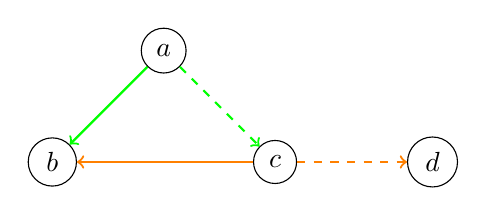
\begin{tikzpicture} [
    node distance={20mm},
    main/.style = {draw, circle},
    s/.style = {->,thick},
    d/.style = {->,thick,dashed}
  ]
  \node[main] (b) {$b$};
  \node[main] (a) [above right of=b] {$a$};
  \node[main] (c) [below right of=a] {$c$};
  \node[main] (d) [right of=c] {$d$};
  \draw[thick,green,->] (a) -- (b);
  \draw[thick,green,->,dashed] (a) -- (c);
  \draw[thick,orange,->] (c) -- (b);
  \draw[thick,orange,->,dashed] (c) -- (d);
\end{tikzpicture}
\caption{Failure of blacklist property}
\label{fig:blacklist}
\end{figure}

Blacklisted nodes are nodes in the network that must not
be reachable.
Let's assume the network in Fig. \ref{fig:blacklist} as
an example where the node $d$ is blacklisted.
For simplicity we assume that we require
$d$ not reachable only from $a$.
Consider the following DyNetKAT program for this network:
\begin{equation*}
\begin{aligned}[c]
    P   & = p!1                             \\
    Q   & = q!1                             \\
    N   & = F \oplus p?1;N_p \oplus q?1;N_q \\
    N_p & = F_p \oplus q?1;F_{pq}           \\
    N_q & = F_q \oplus p?1;F_{pq}           \\
    F   & = a\ra b \oplus c\ra b            \\
\end{aligned}
\qquad\qquad
\begin{aligned}[c]
    F_p         & = a\ra c \oplus c\ra b \oplus a\ra b \\
    F_q         & = a\ra b \oplus c\ra d               \\
    F_{pq}      & = a\ra c \oplus c\ra d \oplus a\ra d \\
    SDN         & = \delta_{\mathcal{L}} (N
    \parallel P \parallel Q)                           \\
    \mathcal{L} & = \set{p!1,p?1,q?1,q?1}                \\
\end{aligned}
\end{equation*}
We assume that there are two concurrent processes for updating
the switches $a$ and $c$.
Let we use $p$ and $q$ to denote $rcfg(p,1)$ and
$rcfg(q,1)$ respectively.
Thus, $p$ and $q$ replace the solid green and orange
paths in the network with dashed paths respectively.

Obviously, executing both $rcfg_{p,1}$ and $rcfg_{q,1}$ leads
to a state where we can forward the $\sigma_a$ to $d$.
To find the cause of error, let $\es = \sem{SDN}$ and $M$
be the causal model of $\es$, where we encode the unsafe behavior 
as:
\begin{equation*}
  \varphi = \exists X \in \conf{\es}.\;\exists e \in X.\;l(e) = a \ra d
\end{equation*}

The property above sets the value of $\varphi$ to True if $\es$ 
contains a configuration with an event labeled $a \ra d$.
In $SDN$ there are two orders of execution for $p$ and $q$; hence,
there are two events for each of these labels in $\es$ 
and thus, there are two events with the label $a \ra d$ as well.
So, let's consider events $p_1,p_2$ with label $p$,
events $q_1,q_2$ with label $q$ and events $ad_1,ad_2$ 
with label $a \ra d$ in $E$. Fig. \ref{fig:blacklist:lattice}
shows a portion of the $\conf{\es}$ lattice, which consists of configurations
which lead to events labeled with $a\ra d$.

\newcommand{\crd}[4][above]{
  \node[draw,circle,inner sep=2pt,fill,label={[#1]:#4}] at (#2,#3) {};
}

\begin{figure}
\centering
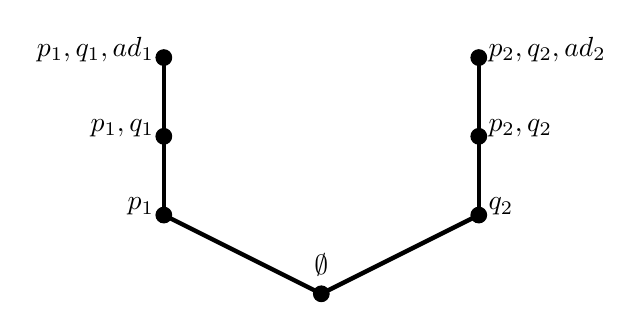
\begin{tikzpicture}
  \crd{0}{0}{$\emptyset$}
  \crd[left]{-2}{1}{$\set{p_1}$}
  \crd[left]{-2}{2}{$\set{p_1,q_1}$}
  \crd[left]{-2}{3}{$\set{p_1,q_1,ad_1}$}
  \crd[right]{2}{1}{$\set{q_2}$}
  \crd[right]{2}{2}{$\set{p_2,q_2}$}
  \crd[right]{2}{3}{$\set{p_2,q_2,ad_2}$}
  \draw [ultra thick] (-2,1) -- (-2,2);
  \draw [ultra thick] (-2,2) -- (-2,3);
  \draw [ultra thick] (0,0) -- (2,1);
  \draw [ultra thick] (0,0) -- (-2,1);
  \draw [ultra thick] (2,1) -- (2,2);
  \draw [ultra thick] (2,1) -- (2,3);
\end{tikzpicture}
\caption{Configurations lattice for the blacklist network}
\label{fig:blacklist:lattice}
\end{figure}


\usetikzlibrary{shapes.geometric}


\begin{figure}
\centering
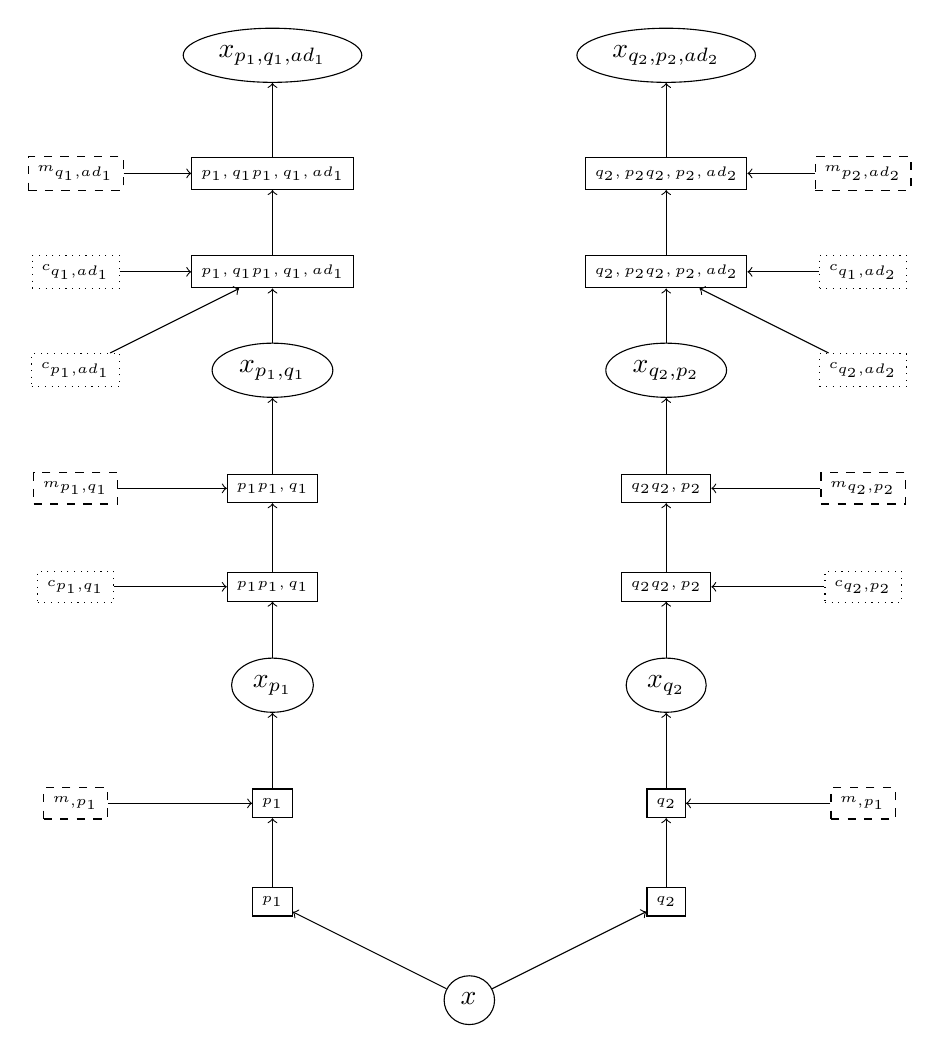
\begin{tikzpicture}
  \tikzset{
    _x/.style={ellipse,draw},
    r/.style={rectangle,draw,font=\tiny},
    m/.style={rectangle,draw,dashed,font=\tiny},
    c/.style={rectangle,draw,dotted,font=\tiny},
  }

  \node[_x] (x-null)    at (0,0)  {$x_{\varnothing}$};
  \node[_x] (x-p1)      at (-2.5,4) {$x_{ \set{p_1} }$};
  \node[_x] (x-p1q1)    at (-2.5,8) {$x_{ \set{p_1,q_1} }$};
  \node[_x] (x-p1q1ad1) at (-2.5,12) {$x_{ \set{p_1,q_1,ad_1} }$};
  \node[_x] (x-q2)      at (2.5,4)  {$x_{ \set{q_2} }$};
  \node[_x] (x-q2p2)    at (2.5,8)  {$x_{ \set{q_2,p_2} }$};
  \node[_x] (x-q2p2ad2) at (2.5,12)  {$x_{ \set{q_2,p_2,ad_2} }$};

  \node[r] (rc-null-p1)      at (-2.5,1.25) {$\rc{\varnothing}{ \set{p_1} }$};
  \node[r] (rm-null-p1)      at (-2.5,2.5) {$\rM{\varnothing}{ \set{p_1} }$};
  \node[r] (rc-p1-p1q1)      at (-2.5,5.25) {$\rc{ \set{p_1} }{ \set{p_1,q_1} }$};
  \node[r] (rm-p1-p1q1)      at (-2.5,6.5) {$\rM{ \set{p_1} }{ \set{p_1,q_1} }$};
  \node[r] (rc-p1q1-p1q1ad1) at (-2.5,9.25) {$\rc{ \set{p_1,q_1} }{ \set{p_1,q_1,ad_1} }$};
  \node[r] (rm-p1q1-p1q1ad1) at (-2.5,10.5) {$\rM{ \set{p_1,q_1} }{ \set{p_1,q_1,ad_1} }$};

  \node[r] (rc-null-q2)      at (2.5,1.25) {$\rc{\varnothing}{ \set{q_2} }$};
  \node[r] (rm-null-q2)      at (2.5,2.5) {$\rM{\varnothing}{ \set{q_2} }$};
  \node[r] (rc-q2-q2p2)      at (2.5,5.25) {$\rc{ \set{q_2} }{ \set{q_2,p_2} }$};
  \node[r] (rm-q2-q2p2)      at (2.5,6.5) {$\rM{ \set{q_2} }{ \set{q_2,p_2} }$};
  \node[r] (rc-q2p2-q2p2ad2) at (2.5,9.25) {$\rc{ \set{q_2,p_2} }{ \set{q_2,p_2,ad_2} }$};
  \node[r] (rm-q2p2-q2p2ad2) at (2.5,10.5) {$\rM{ \set{q_2,p_2} }{ \set{q_2,p_2,ad_2} }$};

  \node[m] (m-null-p1)       at (-5,2.5)  {$m_{\varnothing, p_1 }$};
  \node[m] (m-p1-q1)         at (-5,6.5)  {$m_{\set{p_1}, q_1 }$};
  \node[m] (m-q1-ad1)        at (-5,10.5) {$m_{\set{q_1}, ad_1 }$};

  \node[m] (m-null-q2)       at (5,2.5)  {$m_{\varnothing, p_1 }$};
  \node[m] (m-q2-p2)         at (5,6.5)  {$m_{\set{q_2}, p_2 }$};
  \node[m] (m-p2-ad2)        at (5,10.5) {$m_{\set{p_2}, ad_2 }$};

  \node[c] (c-p1-q1)         at (-5,5.25) {$c_{ p_1,q_1 }$};
  \node[c] (c-p1-ad1)        at (-5,8)    {$c_{ p_1,ad_1 }$};
  \node[c] (c-q1-ad1)        at (-5,9.25) {$c_{ q_1,ad_1 }$};

  \node[c] (c-q2-p2)         at (5,5.25) {$c_{ q_2,p_2 }$};
  \node[c] (c-q2-ad2)        at (5,8)    {$c_{ q_2,ad_2 }$};
  \node[c] (c-p2-ad2)        at (5,9.25) {$c_{ q_1,ad_2 }$};

  \draw[->] (x-null)          -- (rc-null-p1);
  \draw[->] (rc-null-p1)      -- (rm-null-p1);
  \draw[->] (rm-null-p1)      -- (x-p1);
  \draw[->] (x-p1)            -- (rc-p1-p1q1);
  \draw[->] (rc-p1-p1q1)      -- (rm-p1-p1q1);
  \draw[->] (rm-p1-p1q1)      -- (x-p1q1);
  \draw[->] (x-p1q1)          -- (rc-p1q1-p1q1ad1);
  \draw[->] (rc-p1q1-p1q1ad1) -- (rm-p1q1-p1q1ad1);
  \draw[->] (rm-p1q1-p1q1ad1) -- (x-p1q1ad1);
  
  \draw[->] (x-null)          -- (rc-null-q2);
  \draw[->] (rc-null-q2)      -- (rm-null-q2);
  \draw[->] (rm-null-q2)      -- (x-q2);
  \draw[->] (x-q2)            -- (rc-q2-q2p2);
  \draw[->] (rc-q2-q2p2)      -- (rm-q2-q2p2);
  \draw[->] (rm-q2-q2p2)      -- (x-q2p2);
  \draw[->] (x-q2p2)          -- (rc-q2p2-q2p2ad2);
  \draw[->] (rc-q2p2-q2p2ad2) -- (rm-q2p2-q2p2ad2);
  \draw[->] (rm-q2p2-q2p2ad2) -- (x-q2p2ad2);

  \draw[->] (m-null-p1)       -- (rm-null-p1);
  \draw[->] (m-p1-q1)         -- (rm-p1-p1q1);
  \draw[->] (m-q1-ad1)        -- (rm-p1q1-p1q1ad1);

  \draw[->] (m-null-q2)       -- (rm-null-q2);
  \draw[->] (m-q2-p2)         -- (rm-q2-q2p2);
  \draw[->] (m-p2-ad2)        -- (rm-q2p2-q2p2ad2);

  \draw[->] (c-p1-q1)         -- (rc-p1-p1q1);
  \draw[->] (c-p1-ad1)        -- (rc-p1q1-p1q1ad1);
  \draw[->] (c-q1-ad1)        -- (rc-p1q1-p1q1ad1);

  \draw[->] (c-q2-p2)         -- (rc-q2-q2p2);
  \draw[->] (c-q2-ad2)        -- (rc-q2p2-q2p2ad2);
  \draw[->] (c-p2-ad2)        -- (rc-q2p2-q2p2ad2);
\end{tikzpicture}
\caption{Causal graph for the blacklist network}
\label{fig:blacklist:causal-graph}
\end{figure}


The causal graph for this event structure is presented in Fig. \ref{fig:blacklist:causal-graph}.
We claim that $p_1 \cancel{\#} q_1$ is a cause of $\varphi$. To check, we only need to see
if there is a path from $c_{p_1,q_1}$ to either $x_{p_1,q_1,ad_1}$ or $x_{q_2,p_2,ad_2}$.
In this case, there is such a path; so the causality claim holds.
$q_2 \cancel{\#} p_2$ is also a cause of $\varphi$, due to symmetry.
\end{exmp}